
\documentclass[a4paper,10pt]{article}


\usepackage{graphicx}
\usepackage{float}
\usepackage{amsmath}
\usepackage{color}
\usepackage{pdfpages}


\usepackage[latin1]{inputenc}

\usepackage[spanish]{babel}



\title{		\textbf{Trabajo Pr�ctico Final}}


\author{	Bruno, Tom�s ; \textit{Padr�n Nro. 88.449}                     \\
            \texttt{ tbruno88@gmail.com }                                              \\
			Ferreiro, Demian ; \textit{Padr�n Nro. 88443}               						      \\
            \texttt{ epidemian@gmail.com }                                              \\	
			Leguizamo, Mat�as ; \textit{Padr�n Nro. }                     \\
            \texttt{ matias.leguizamo@gmail.com }                                              \\	
            Mouso, Nicol�s ; \textit{Padr�n Nro. 88.528}                     \\
            \texttt{ nicolasgnr@gmail.com }                                              \\[2.5ex]
            \normalsize{Ayudante: Emiliano Ritiro}                       \\
			\normalsize{1er. Cuatrimestre de 2010}                       \\
            \normalsize{75.10 Tecnicas de Dise�o}                    	\\
            \normalsize{Facultad de Ingenier�a, Universidad de Buenos Aires}            \\
       }
\date{}



\begin{document}

% Inserta el t�tulo.
\maketitle

% Quita el n�mero en la primer p�gina.
\thispagestyle{empty}



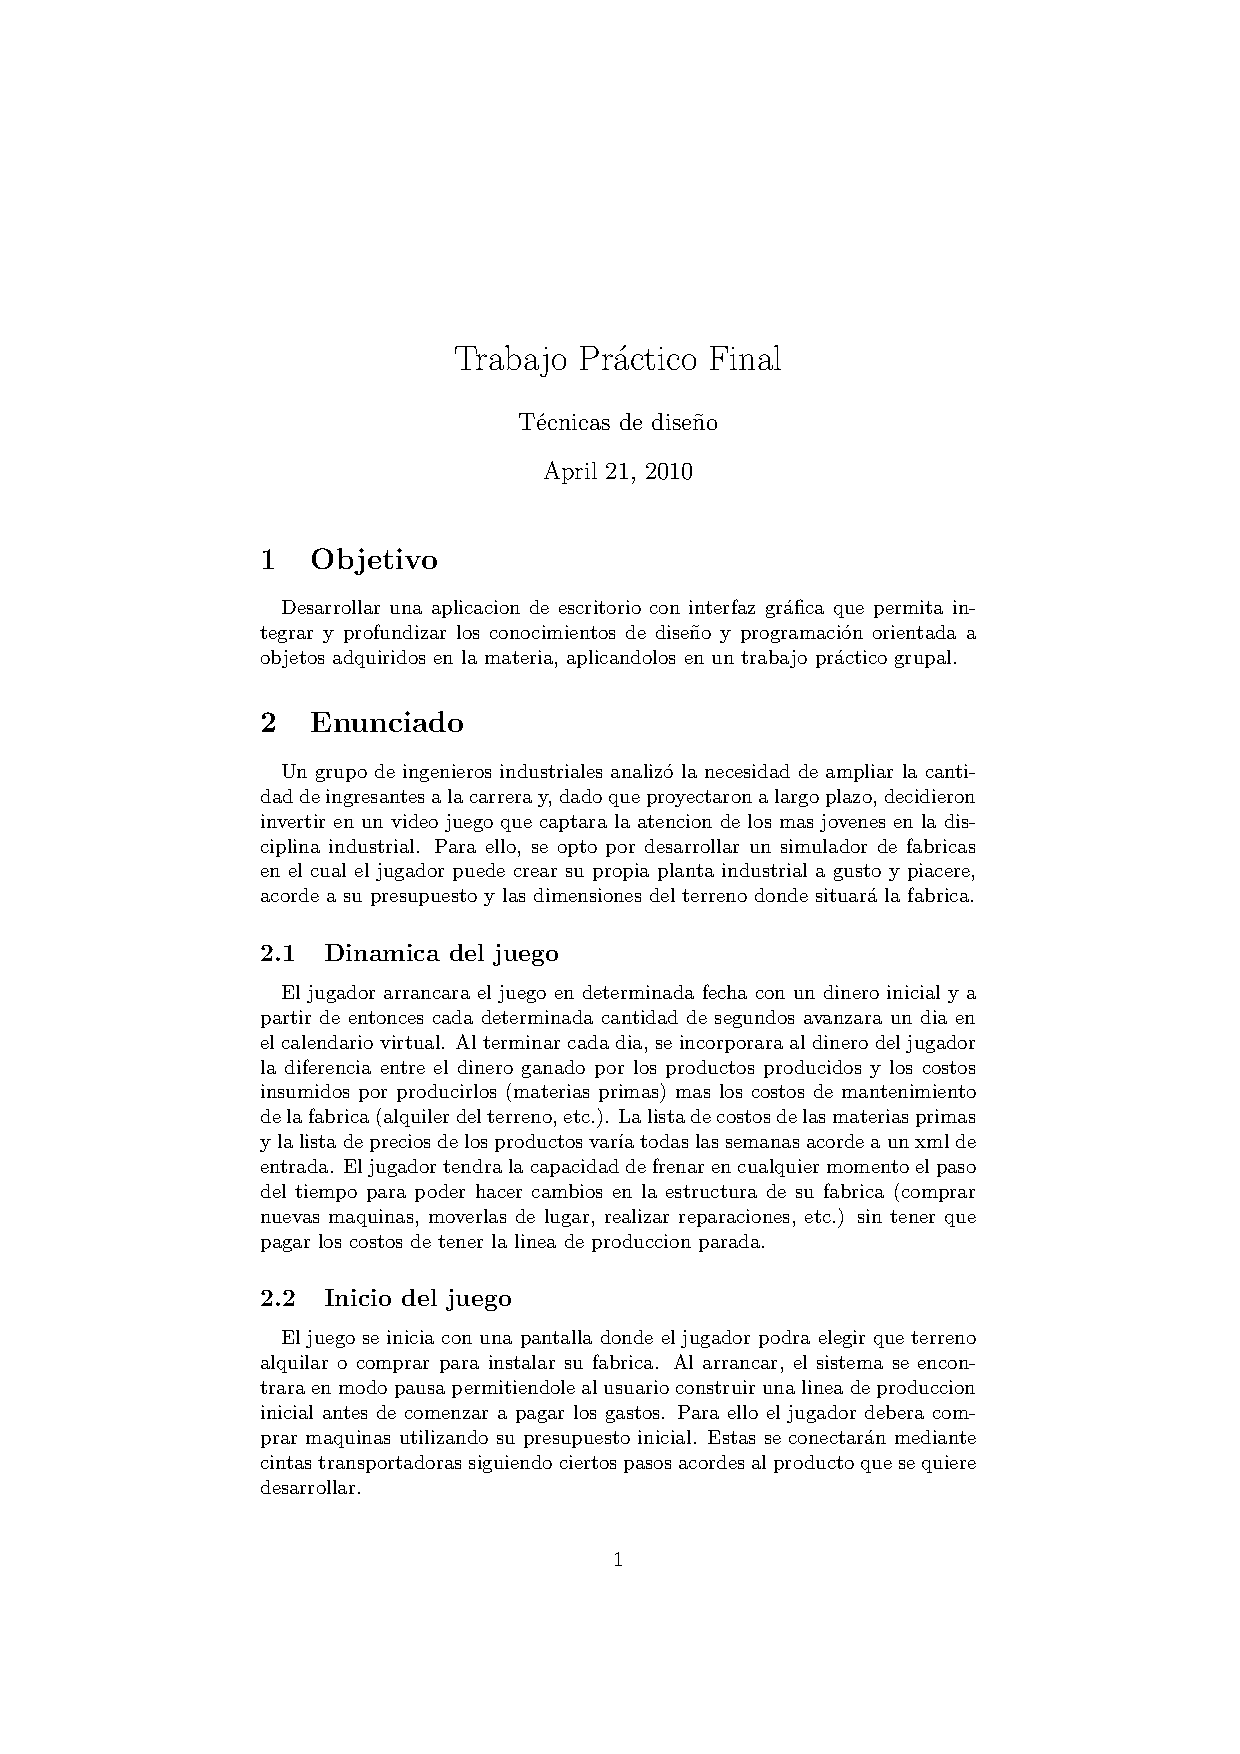
\includepdf[pages={1,2,3,4}]{enunciado.pdf}

\clearpage
\tableofcontents
\setcounter{page}{5}

\clearpage
\section{Hipot�sis}

	\begin{enumerate}
		\item Las m�quinas se pueden reparar por separado o se puede reparar toda una l�nea al mismo tiempo
		\item Se pueden romper tanto las m�quinas de control de calidad como las que son exclusivamente para la producci�n.
		\item Tanto los precios de la materia prima como los de los productos var�an todas las semanas. El resto de los precios se mantiene invariante en el tiempo
		\item Las paredes no pueden ser borradas ni vendidas del terreno adquirido.
		\item Los productos son construidos a partir de distintos tipos de materias primas y de cantidades de cada una de estas. 
			Pueden suceder que existan dos l\'ineas de producci\'on que pese a tener una misma secuencia de producci\'on, tengan como resultado productos distintos como consecuencia de tener una entrada de materia prima distinta.
		\item Para poder producir, cada l\'inea de producci\'on debe estar conectada a una salida de la fabrica.
		\item El precio de alquiler de la fabrica es proporcional al precio del terreno.
		\item Las maquinas pueden no contener una entrada y una salida determinada en el archivo XML. En caso de que no tengan una establecida entonces se les genera una por defecto.
		\item Tanto las salidas como las paredes de las fabricas se encuentran declaradas en el archivo XML correspodiente a los distintos terrenos.
		\item Las m\'aquinas de control de calidad pueden convertir a un producto en defectuoso.
		\item Puede suceder que un mismo tipo de producto sea creado a partir de distintas secuencias de producci\'on y diferentes materiales.
	\end{enumerate}

\clearpage
\section{Vista L�gica}
	\subsection{Producci�n}
		
		La forma en la cual el juego simula la producci\'on es el n\'ucleo del modelo. 

		La primer decisi\'on de relevancia fue si en el juego cada producto iba a ser un objeto que fuera circulando por cada maquina o si simplemente al final del d\'ia se discretizar\''ia la producci\'on diaria. Decidimos optar por la primer alternativa porque consideramos que la segunda alternativa no representaba correctamente al negocio. Aunque se podr\'ian modelizar las funcionalidades solicitadas en el presente, cada futuro cambio llevar\'ia a nuevos parches con peligro de tener que desechar el n\'ucleo del modelo por completo en caso de que no quedara otra alternativa. La segunda alternativa probablemente ser\'ia una buena opci\'on en caso de que se tuvieran que manejar varias fabricas simult�neamente.
		
		Una vez decidido acerca de la existencia fisica de cada producto, se abrieron distintos interrogantes. Un ejemplo fue la forma en la cual se identificar\'ia el producto luego de ser procesado por las distintas m\'aquinas.
		
		La primera alternativa que se considero fue que cada l\'inea fuera la encargada de identificar el tipo de producto que produc\'ia. Esto parec\'ia l\'ogico ya que la l\'inea sabe las m\'aquinas que tiene. Sin embargo, identificamos una limitaci\'on en esta soluci\'on. Esta limitaci\'on surg\'ia de que cada vez que modificaramos las m\'aquinas de la l\'inea, los productos que estuvieran siendo procesados en ese momento en la l\'inea podr\'ian terminar resolviendo su tipo incorrectamente. 
		
		En consecuencia, decidimos que cada producto lleve un historial de las m\'aquinas por las que pasaba. Al final de ser procesado por todas las m\'aquinas, se analizaba cual era el producto final.
			
		Con el objetivo de aumentar el interes al momento de jugarlo, decidimos tomar como hipot\'esis que el producto puede necesitar distintas materias primas y cantidades de cada una de ellas. 
		
		En el diagrama de clases se puede observar a grandes rasgos como se implement\'o la decisi�n de que cada producto guarda un historial: cada producto cuando es procesado por una maquina guarda la informaci�n acerca del tipo de maquina por el que fue procesado adem�s de la materia de prima con la que fue creado . Para que esto sea realizado, existe un m�todo process que esta redefinido en los distintos tipos de productionLineElements.
		
		\begin{figure}[H]
		\centering
		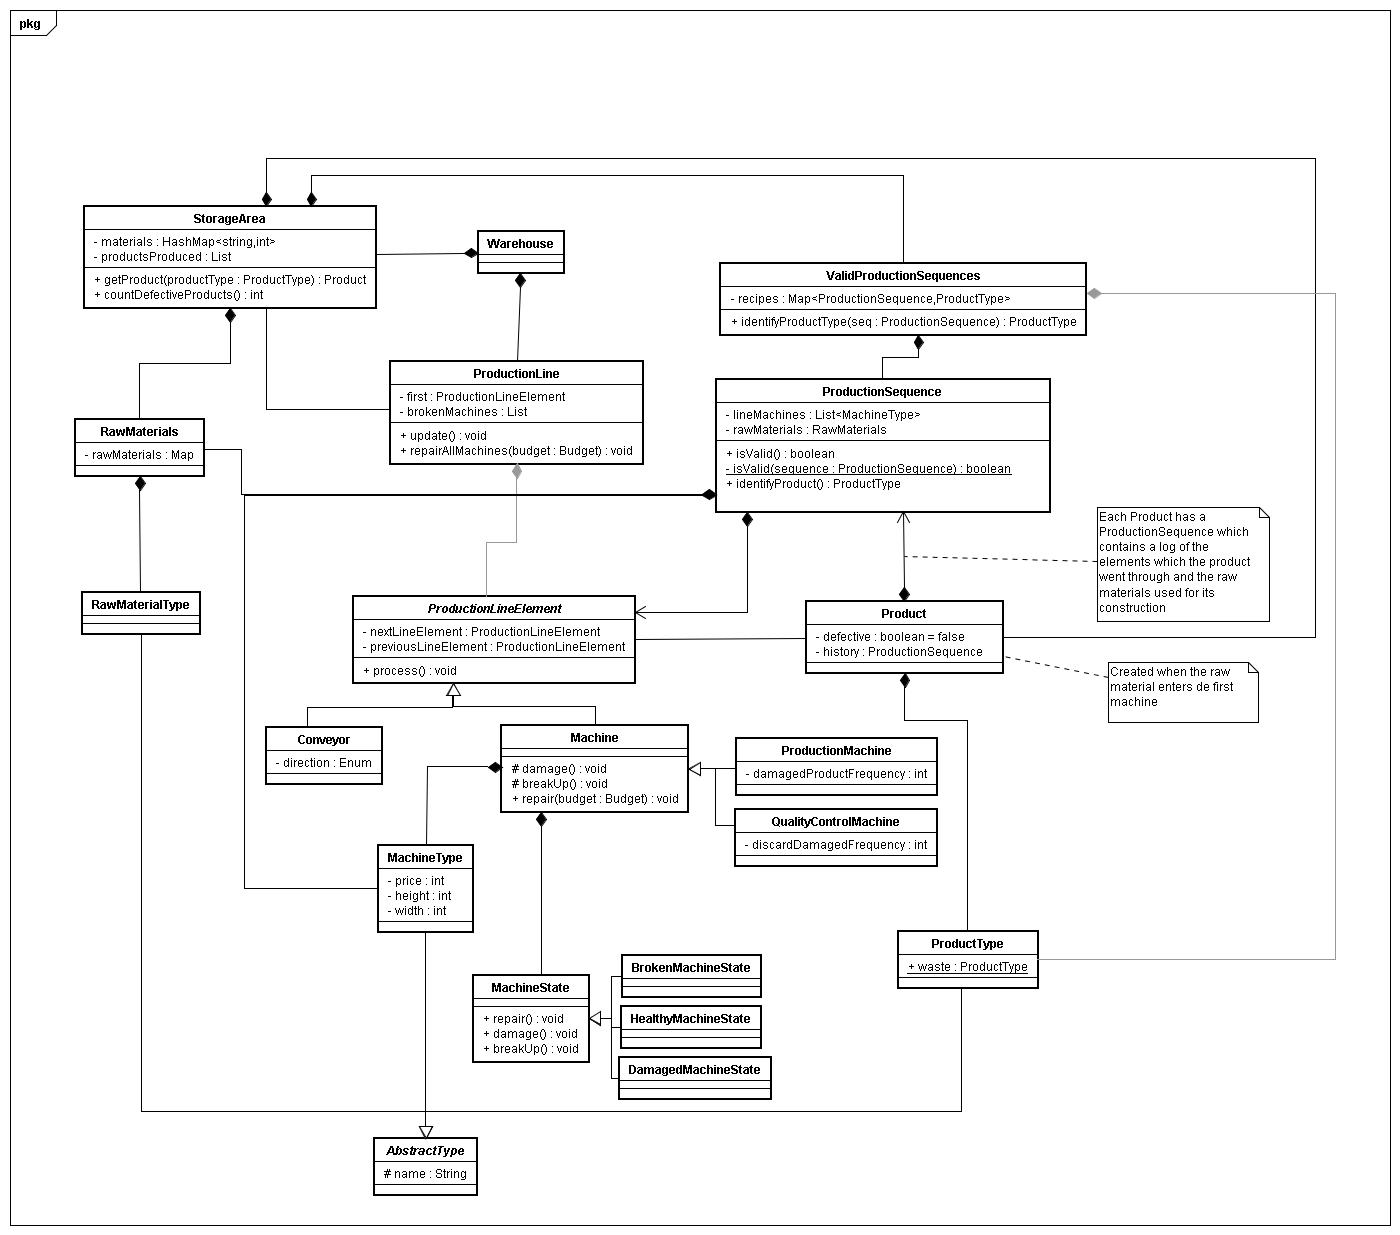
\includegraphics[scale=0.5]{diagramas/productionClassDiagram.jpg}
		\caption{Diagrama de Clases de la l�gica de producci�n}
		\end{figure}		
		
				
		En el diagrama de secuencia, se puede observar como es la secuencia desde que sea crea un producto amorfo, que no sabe que tipo de producto es,  hasta que finalmente se resuelve su tipo. En el interin, el producto es procesado por todos los distintos elementos que forman parte de la l\'inea de producci\'on.

	
		\begin{figure}[H]
		\centering
		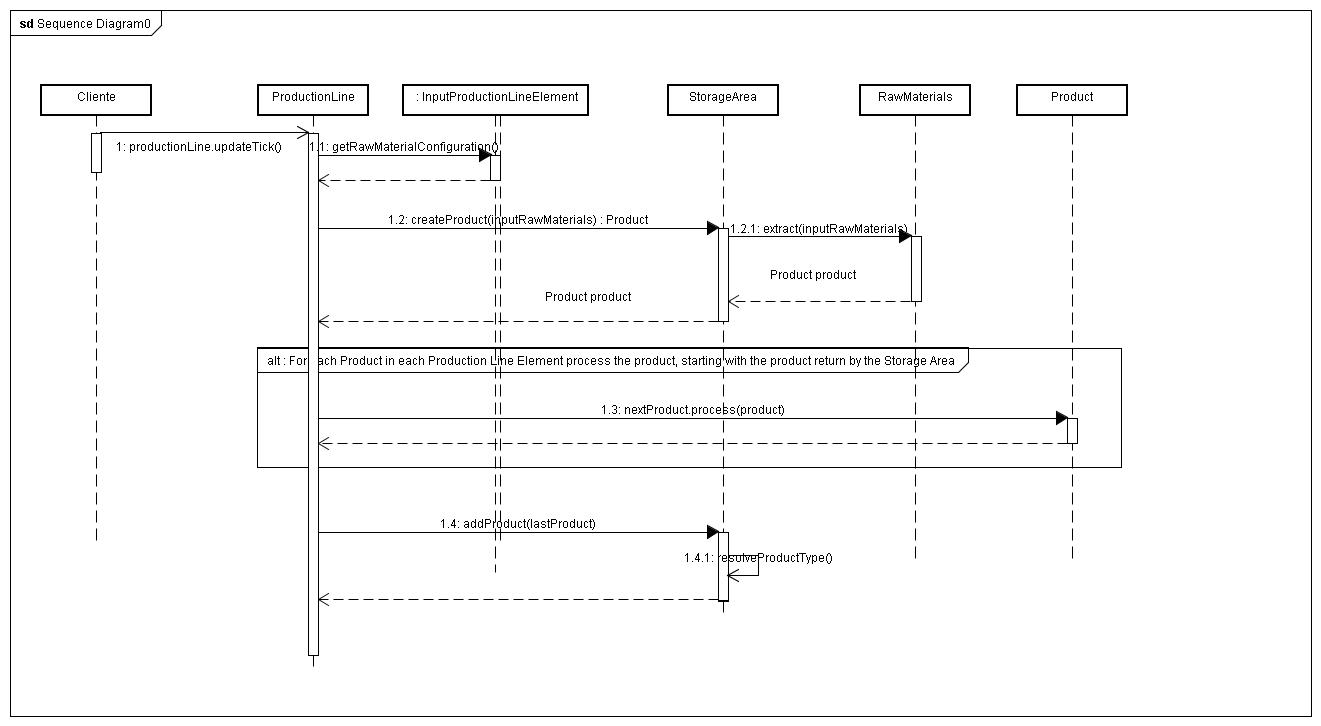
\includegraphics[scale=0.5]{diagramas/productionSequenceDiagramBis.jpg}
		\caption{Diagrama de Secuencia de la l�gica de producci�n}
		\end{figure}		

	\subsection{Discretizaci\'on Temporal }		
		Como se pod\'ia observar en el grafico , existe un metodo en la l\'nea de producci\'on que dispara la circulaci\'on del producto a trav\'es de las m\'aquinas. En cada ``tick'', un producto pasa de una maquinaa la siguiente.
		De la misma forma, existen otras entidades que se suscriben a una entidad que se encarga de actualizar el paso del tiempo en todos los objetos que esten suscriptos a ella.
		Cada d\'ia esta formado por una cantidad especificada de ticks. 
A su vez, la cantidad de d\'ias por semana y d\'ias por mes tamb\'ien se encuentra parametizada.
		
	\subsection{Laboratorio de Tecnolog�as}
		
		El laboratorio se ocupa de desarrollar las distintas secuencias de producci\'on que resultan en productos validos. Cada desarrollo que realiza el laboratorio se considera una \emph{tecnolog\'ia} y cada una de las cuales habilita o una nueva forma de producir un producto o un producto nuevo.  
		
		Al momento de dise\~nar el laboratorio se busco que el laboratorio no sea algo secundario y prescindible. As\'i fue que se decidio que las tecnolog\'ias que este desarrolla tengan una estructura jerarquica en la cual cada tecnolog\'ia puede tener dependencias. Es decir, que se necesite desarrollar otras tecnolog\'ias antes de esta.
		
		
		\begin{figure}[H]
		\centering
		\includegraphics[scale=0.4]{diagramas/TechnologyClassDiagram.jpg}
		\caption{Diagrama de Clases de la l�gica del desarrollo de Tecnolog�as}
		\end{figure}	
		
	\subsection{Arquitectura General}
		
		\begin{figure}[H]
		\centering
		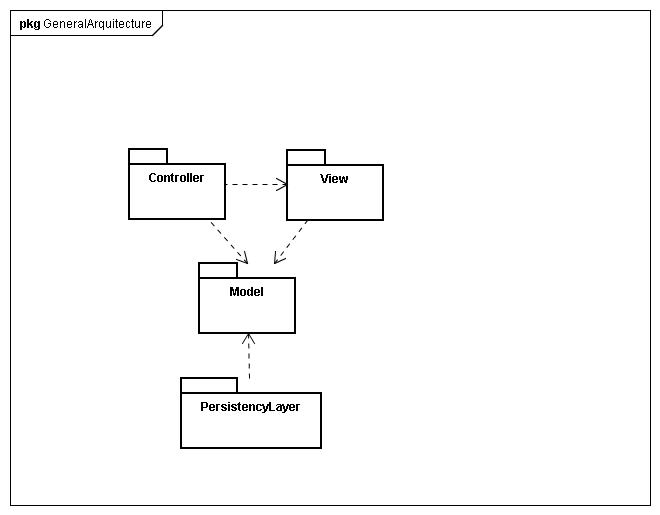
\includegraphics[scale=0.5]{diagramas/generalArchitecture.jpg}
		\caption{Diagrama de Paqutes general de la Arquitectura}
		\end{figure}	
		
		La arquitectura sigue al patr\'on de arquitectura, \emph{MVC}. El modelo no depende de nada m\'as que si mismo, Los controladores utilizan al modelo y a la vista y la vista necesita del modelo. La capa de persistencia tambi\'en esta desacoplada completamente del modelo.
		
	\subsection{Persistencia}
		
		\begin{figure}[H]
		\centering
		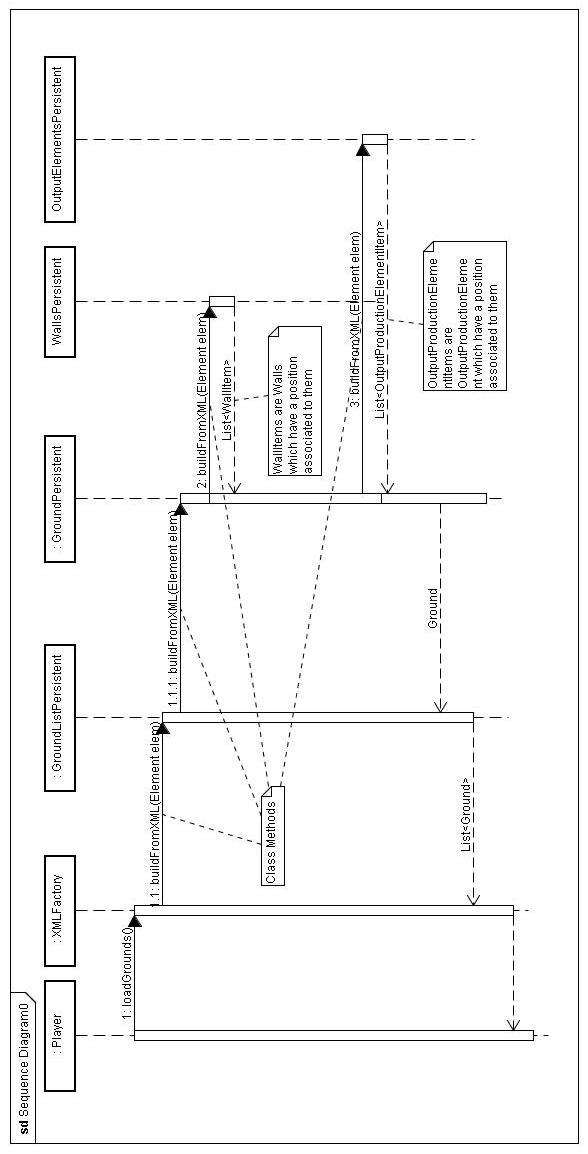
\includegraphics[scale=0.7]{diagramas/SequenceDiagramPersistence.jpg}
		\caption{Diagrama de Secuencia de la recuperaci\'on de archivos XML}
		\end{figure}	
		
		\begin{figure}[H]
		\centering
		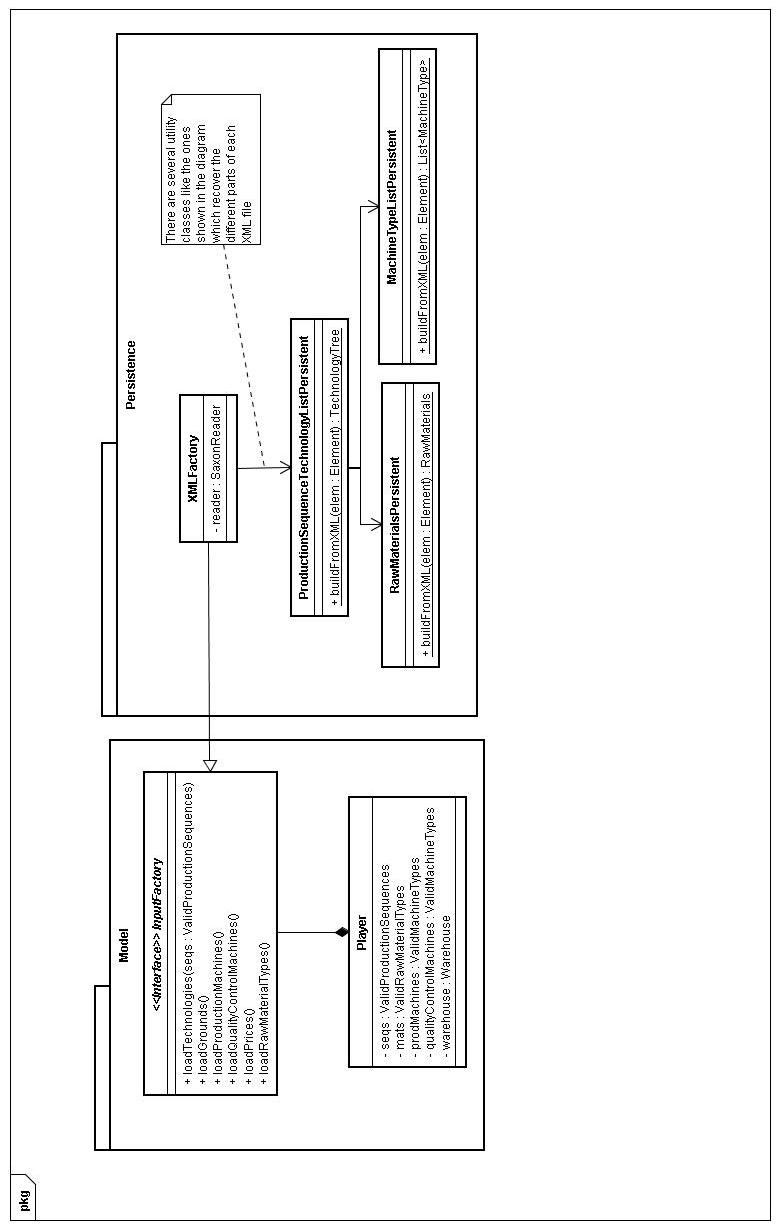
\includegraphics[scale=0.7]{diagramas/persistenceCD.jpg}
		\caption{Diagrama de Clases general de la persistencia}
		\end{figure}	

\clearpage
\section{Vista de Desarrollo}
	
	\begin{figure}[H]
	\centering
	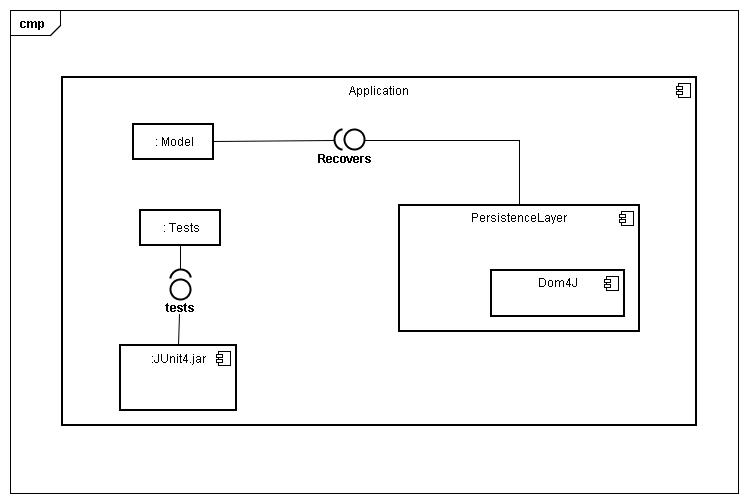
\includegraphics[scale=0.5]{diagramas/componentDiagram.jpg}
	\caption{Diagrama de Componentes}
	\end{figure}
	
	En la implementaci\'on de la capa de recuperaci\'on de datos a la que llamamos persistencia por una posible futura extensi\'on, se utiliz\'o un componente para facilitar la recuperaci\'on.   
	
	El componente que utilizamos es la libreria Dom4j. La utilizaci\'on de esta libreria nos permitio desligarnos de la necesidad de hacer un parser de XML.
	
	Otro componente que utilizamos durante el desarrollo fue el framework JUnit. La utilizaci\'on de este framework facilito la construcci\'on de pruebas que nos sirvieron en primer lugar para ir probando los distintos modulos que se iban implementando y en segundo lugar, para poder refactorizarlos sin miedo a meter nuevas fallas en el programa. 

\clearpage
\section{Vista de Procesos}

	La aplicaci\'on corre en una computadora, sobre una Java Virtual Machine. Dentro de esta maquina virtual corre un \'unico proceso. No existe comunicaci\'on alguna de este proceso con otros procesos.
	
	\begin{figure}[H]
	\centering
	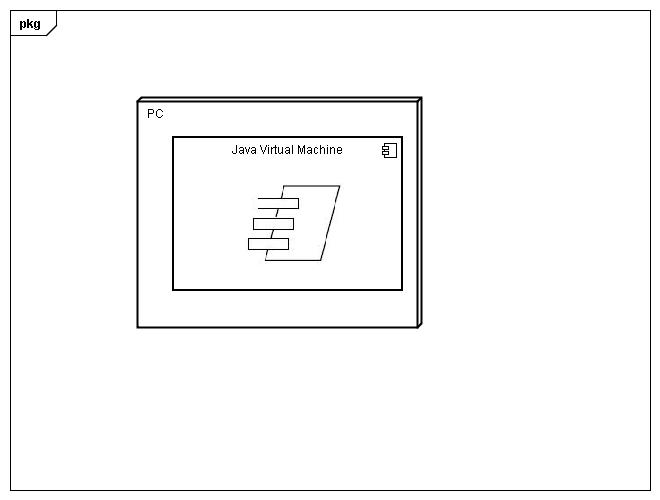
\includegraphics[scale=0.5]{diagramas/processDiagram.jpg}
	\caption{Diagrama de Procesos }
	\end{figure}
	
	En una aplicaci\'on como la desarrollada, la complejidad de la vista de procesos es muy simple en comparaci\'on al de la vista l\'ogica o de desarrollo
	
\clearpage
\section{Vista F�sica}
	\begin{figure}[H]
	\centering
	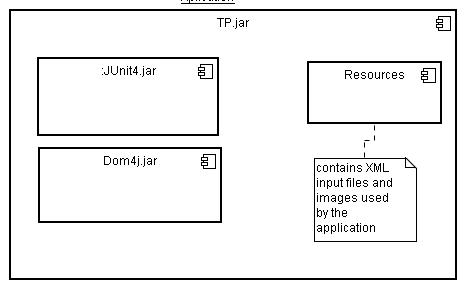
\includegraphics[scale=0.5]{diagramas/deployment24.jpg}
	\caption{Diagrama de Despliegue }
	\end{figure}
	
	El diagrama de \emph{deployment} es muy simple ya que la aplicaci\'on no es una aplicaci\'on que este desplegada en m\'as de un sistema. Por lo tanto, todos los componentes existentes estan contenidos en el \'unico nodo del sistema.
	
	Adem\'as, se puede observar que el jar de la aplicaci\'on contiene dentro de si a los jars de los otros componentes necesarios para el uso del programa. Esto simplifica la instalaci\'on del programa ya que no tendra que lidiar con problemas de dependencias. Tiene como desventaja que el usuario puede llegar a tener que tener estas librerias m\'as de una vez en su computadora.
	
\clearpage
\section{Escenarios}

	\begin{figure}[H]
	\centering
	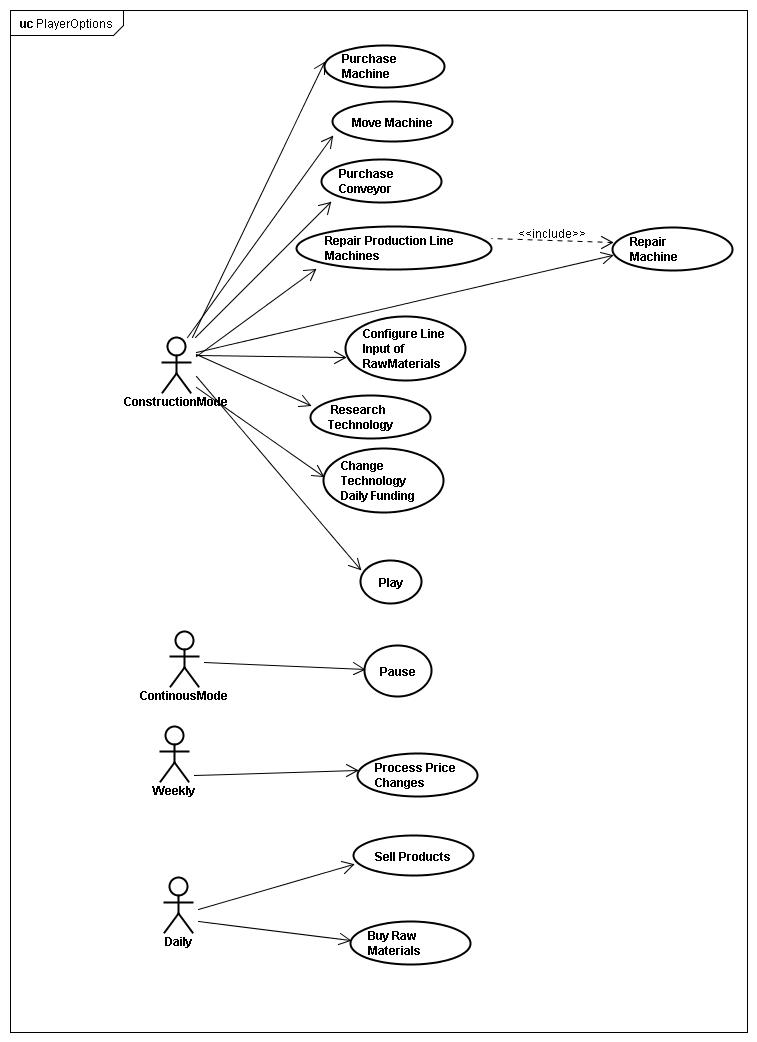
\includegraphics[scale=0.5]{diagramas/useCase.jpg}
	\caption{Diagrama de Casos de Uso}
	\end{figure}			
	
	\subsection{Funcionalidades}
	
		\begin{enumerate}
			
			\item{\emph{ Purchase Machine:}} El jugador puede comprar m\'aquinas y ubicarlas en la fabrica.
			
			\item{\emph{ Purchase Conveyor:}}  El jugador puede colocar segmentos de cintas transportadoras. Una vez conectadas las cintas transportadoras con otros elementos de la l\'inea, la cinta muestra la direcci\'on que seguira el producto. Acci\'on ejecutada desde el modo construcci\'on.
			
			\item{\emph{ Sell Warehouse:}} El jugador puede vender la fabrica y volver a la selecci\'on de terrenos.
			
			\item{\emph{ Sell Machine:}} El jugador puede vender la maquinay recibir a cambio un valor proporcional de su precio consecuencia de la depreciaci\'on sufrida.
			
			\item{\emph{ Move Machine:}}  El jugador puede reubicar m\'aquinas ya compradas en las distintas ubicaciones disponibles de la fabrica. La maquinaqueda ubicada en la fabrica con su respectiva entrada y salida. 
		
			\item{\emph{ Configure Input of Raw Materials:}} El jugador selecciona la materia prima que se usara para la producci\'on en la l\'inea. 
		
			\item{\emph{ Repair Production Line Machines:}} El jugador selecciona la linea de producci\'on cuyas m\'aquinas desea reparar. La reparaci\'on tiene un costo proporcional al precio de la m\'aquina. Acci\'on ejecutada desde el modo construcci\'on.
			
			\item{\emph{ Repair Machine:}} El jugador repara una maquinaque selecciona. La reparaci\'on tiene un costo proporcional al precio de la m\'aquina. Acci\'on ejecutada desde el modo construcci\'on.
			
			\item{\emph{ Play:}} El jugador pasa a modo continuo.
			
			\item{\emph{ Pause:}} El jugador pasa a modo construcci\'on. Desde el modo construcci\'on. 
			
			\item{\emph{ Process prices change:}} Semanalmente cambian todos los precios de los productos y las materias primas.
			
			\item{\emph{ Sell Products:}} Al final de cada d\'ia, la producci\'on es vendida con los precios correspondientes a esa semana.
			
			\item{\emph{ Buy Raw Materials:}}  El jugador compra la materia prima que quiera. Acci\'on ejecutada desde el modo construcci\'on.
			
			\item{\emph{ Research Technology:}} El jugador decide cual ser\'a la pr\'oxima tecnolog\'ia que sera desarrollada
			
			\item{\emph{ Change Technology Daily Funding:}} El jugador establece cuanta plata invertir\'a en el desarrollo de nuevas tecnolog\'ias.
		
		\end{enumerate}

\clearpage	
\section{Posibles Mejoras y Extensiones}
	Una funcionalidad que nos hubiera gustado poder implementar es el hecho de que el jugador pueda solicitar prestamos para que no pierda apen\'as se queda sin plata.
	
	
		
\clearpage	
\section{Conclusi\'on}	
	La primer conclusi\'on a la que llegamos fue que en reiteradas ocasiones tomamos decisiones que aumentaban la complejidad del sistema sin hacer un an\'alisis completo de si pod\'iamos llegar a implementarlas a tiempo. As\'i fue que durante las \'ultimas semanas de desarrollo nos encontramos muy apretados por el tiempo incluso habiendo aprovechado todas las semanas que nos hab\'ian provisto para el desarrollo del mismo.
	
	Una segunda conclusi\'on es que es preferible tomarse el tiempo necesario para dise\~narlo bien el sistema antes de empezar a escribir c\'odigo. No hacerlo puede resultar en perder mucho tiempo en caso de que como consecuencia de un requisito que no se hab\'ia contemplado o una idea que no se hab\'ia terminado de cerrar, sea necesario replantearse el problema. 
	
\clearpage
\begin{thebibliography}{9}
  \bibitem{ieee} KRUCHTEN, Philipe. ``Architectural Blueprints $\-$ The \emph{4+1} View Model of Software Architecture''
  \bibitem{wiki} Wikipedia EN, ``4+1 Architectural View Model''
\end{thebibliography}

\end{document}

